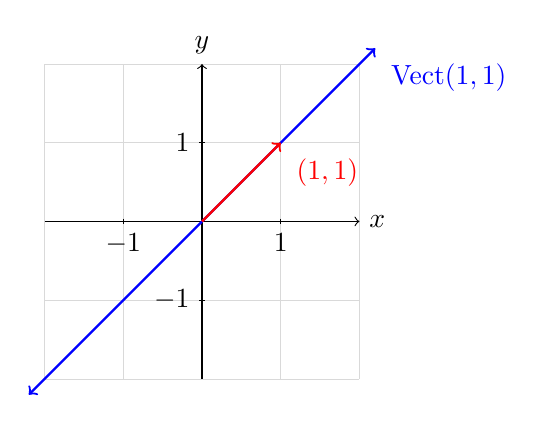
\begin{tikzpicture}[scale=1]
	% Grille de fond
	\draw[very thin,gray!30] (-2,-2) grid (2,2);
	
	% Axes
	\draw[->] (-2,0) -- (2,0) node[right] {$x$};
	\draw[->] (0,-2) -- (0,2) node[above] {$y$};
	
	% Graduations principales
	\foreach \x in {-1,1}
	{
		\draw (\x cm,1pt) -- (\x cm,-1pt) node[anchor=north] {$\x$};
		\draw (1pt,\x cm) -- (-1pt,\x cm) node[anchor=east] {$\x$};
	}
	
	% Droite vectorielle en bleu
	\draw[<->,blue, thick] (-2.2,-2.2) -- (2.2,2.2) node[below right = 2pt] {$\textcolor{blue}{\textup{Vect}(1,1)}$};
	
	% Vecteur (1,1) en rouge avec étiquette plus basse
	\draw[->, red, thick] (0,0) -- (1,1) node[below right=2pt] {$(1,1)$};
\end{tikzpicture}